\documentclass[a4paper, fontsize = 14pt]{article}
\usepackage{hyperref}
\usepackage[warn]{mathtext}
\usepackage[english,russian]{babel}
\usepackage[utf8x]{inputenc} 
 
%математика
\usepackage[mathscr]{eucal}
\usepackage{amsmath,amsfonts,amssymb,amsthm,mathtools}
\usepackage{icomma}
\usepackage{wasysym}
\usepackage{mathrsfs}
\usepackage[italicdiff]{physics}
 
%оформление текста
\usepackage{setspace}
\onehalfspacing
\usepackage{indentfirst}
\usepackage{scrextend}
 
%геометрия
\usepackage{geometry}
\geometry{left=25mm,right=25mm,
 top=25mm,bottom=30mm}
 
%графика
\usepackage{wrapfig}
\usepackage{graphicx}
\usepackage{pgfplots}
\usepackage{tikz}
\RequirePackage{caption}
\DeclareCaptionLabelSeparator{defffis}{ --- }
\captionsetup{justification=centering,labelsep=defffis}
 
%таблицы
\usepackage{array,tabularx,tabulary,booktabs} 
\usepackage{longtable}  
\usepackage{multirow} 
 
%ссылки
\usepackage{hyperref}
\usepackage{xcolor}
\definecolor{grn}{HTML}{57A14F} %зеленый
\definecolor{rd}{HTML}{E53C44} %красный 
\definecolor{bl}{HTML}{282691} %синий 
\definecolor{bbl}{HTML}{001B6C} %темно-синий
\hypersetup{		
    colorlinks=true,       	
    linkcolor=bbl,          % внутренние ссылки
    citecolor=rd,          % на библиографию
    filecolor=magenta,      % на файлы
    urlcolor=bl           %внешние источники
}
 
% Колонтитулы
\usepackage{fancyhdr} 
 	\pagestyle{fancy}
 	\renewcommand{\headrulewidth}{0.15mm}  
 	\renewcommand{\footrulewidth}{0.15mm}
 	\lfoot{№2.1.6 Эффект Джоуля-Томсона}
 	\rfoot{\thepage}
 	\cfoot{}
 	\rhead{}
 	\chead{}
 	\lhead{Мещеряков Всеволод, Б02-001}
 
 
\begin{document}

\begin{center} \textbf{
Лабораторная работа №2.1.6 \\ Эффект Джоуля-Томсона \\
Мещеряков Всеволод, Б02-001, 22.04.2021}
\end{center} 

\subsection*{Введение}

Цель работы заключается в определении изменения температуры углекислого газа при протекании через малопроницаемую перегородку при разных начальных значениях давления и температуры. После определения зависимости вычисляются коэффициенты Ван-дер-Ваальса "a" и "b".

Для этого в работе используются трубка с пористой перегородкой, труба Дьюара, термостат, термометры, дифференциальная термопара, микровольтметр, балластный баллон, манометр.

\subsection*{Теоретическая справка}

В работе рассматривается дифференциальный эффект Джоуля-Томсона, то есть когда изменения давления и температуры малы. В этом случае коэффициент Джоуля-Томсона $\mu_{д-т}$, равный отношению перепада температур к перепаду давления, приблизительно равен производной температуры по давлению при постоянной энтальпии. С учетом постоянства энтальпии и ее зависимости только от температуры и давления получаем:

\begin{equation}
	\mu_{д-т}=\frac{\Delta T}{\Delta P}\approx (\pdv{T}{P})_{H} = -\frac{(\pdv{H}{P})_T}{(\pdv{H}{T})_P}.
\end{equation}

Пользуясь соотношениями для полных дифференциалов термодинамических потенциалов, окончательно получаем выражение для коэффициента Джоуля-Томсона:

\begin{equation}
	\mu_{д-т}=\frac{T(\pdv{V}{T})_P-V}{C_p}.
\end{equation}

Для газа Ван-дер-Ваальса выражение принимает вид:

\begin{equation}
	\mu_{д-т}=\frac{\Delta T}{\Delta P}\approx \frac{\frac{2a}{RT}-b}{C_p}.
\end{equation}

\subsection*{Ход работы}

При фиксированной температуре термостата будем менять величину перепада давления и снимать зависимость перепада температур газа. Результаты отразим в таблице 1 приложения. Так же построим графики перепада давления температуры от перепада давления - рисунки 2, 4, 5 приложения.

Из графиков получим значения коэффициентов наклона, которые в свою очередь равны коэффициентам Джоуля-Томсона при данных температурах:

\[\mu_{д-т|293}=k_{293} = (911\pm46)\cdot 10^{-3} (К/атм),\] \[ \mu_{д-т|303}
=k_{303} = (906\pm58)\cdot 10^{-3} (К/атм),\] \[ \mu_{д-т|313}=k_{313} = (803\pm45)\cdot 10^{-3} (К/атм)\] 

Отсюда получаем значения коэффициентов из уравнения Ван-дер-Ваальса для исследуемого газа $CO_2$:

\[ a = \frac{(\mu_{д-т|293} - \mu_{д-т|303})\cdot C_p \cdot T_{293} T_{303}}{2R\cdot(T_{303}-T_{293})}=0,055(Н\cdot м^4/ моль^2) \]

\[ b = \frac{2\cdot a}{RT_{293}} - \mu_{д-т|293}\cdot C_p = 0,018(м^3/моль) \]

\newpage

\subsection*{Приложение}

\begin{table}[hbt]
\centering
\caption{\textit{Показания установки при разных температурах термостата}}
\scalebox{1.2}{
\begin{tabular}{|c|c|c|c|c|c|}
\hline
\multicolumn{6}{|c|}{\textbf{T = 293 К}}                             \\ \hline
\textbf{$\Delta P, атм$}          & 4,3  & 4    & 3,5  & 3    & 2,5  \\ \hline
\textbf{$\sigma_{\Delta P}, атм$} & 0,1  & 0,1  & 0,1  & 0,1  & 0,1  \\ \hline
\textbf{$\Delta U, мкВ$}          & 135  & 125  & 107  & 84   & 72   \\ \hline
\textbf{$\sigma_{\Delta U}, мкВ$} & 2    & 2    & 2    & 2    & 2    \\ \hline
\textbf{$\Delta T, к$}            & 3,39 & 3,14 & 2,67 & 2,11 & 1,81 \\ \hline
\textbf{$\sigma_{\Delta T}, К$}   & 0,05 & 0,05 & 0,05 & 0,05 & 0,05 \\ \hline
\multicolumn{6}{|c|}{\textbf{T = 303 К}}                             \\ \hline
\textbf{$\Delta P, атм$}          & 4,2  & 4    & 3,5  & 3    & 2,5  \\ \hline
\textbf{$\sigma_{\Delta P}, атм$} & 0,1  & 0,1  & 0,1  & 0,1  & 0,1  \\ \hline
\textbf{$\Delta U, мкВ$}          & 131  & 121  & 101  & 85   & 67   \\ \hline
\textbf{$\sigma_{\Delta U}, мкВ$} & 2    & 2    & 2    & 2    & 2    \\ \hline
\textbf{$\Delta T, к$}            & 3,22 & 2,98 & 2,48 & 2,09 & 1,65 \\ \hline
\textbf{$\sigma_{\Delta T}, К$}   & 0,05 & 0,05 & 0,05 & 0,05 & 0,05 \\ \hline
\multicolumn{6}{|c|}{\textbf{T = 313 К}}                             \\ \hline
\textbf{$\Delta P, атм$}          & 4,3  & 4    & 3,5  & 3    & 2,6  \\ \hline
\textbf{$\sigma_{\Delta P}, атм$} & 0,1  & 0,1  & 0,1  & 0,1  & 0,1  \\ \hline
\textbf{$\Delta U, мкВ$}          & 129  & 116  & 100  & 83   & 72   \\ \hline
\textbf{$\sigma_{\Delta U}, мкВ$} & 2    & 2    & 2    & 2    & 2    \\ \hline
\textbf{$\Delta T, к$}            & 3,11 & 2,79 & 2,41 & 1,99 & 1,73 \\ \hline
\textbf{$\sigma_{\Delta T}, К$}   & 0,05 & 0,05 & 0,05 & 0,05 & 0,05 \\ \hline
\end{tabular}
}
\end{table}

\begin{figure}[hbt]
\center{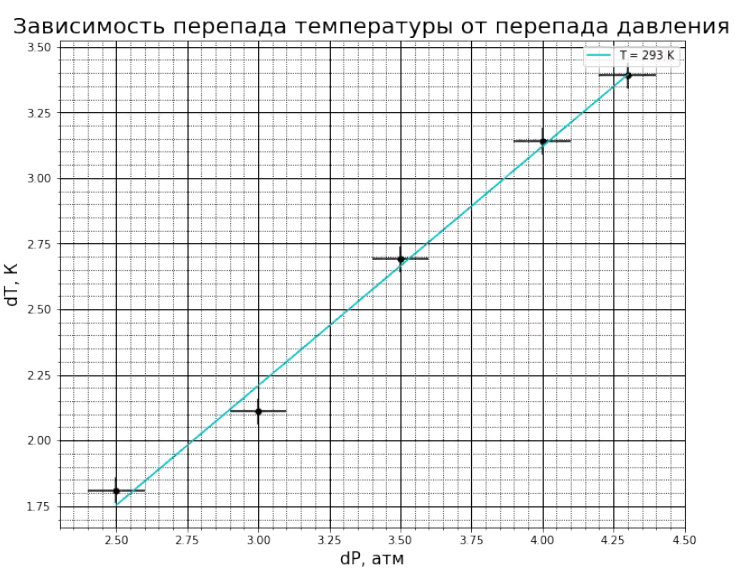
\includegraphics[scale=0.9]{lab216ris2.png}}
\caption{\textit{Зависимость перепада температуры от перепада давления при 293К}}
\end{figure}

\begin{figure}[hbt]
\center{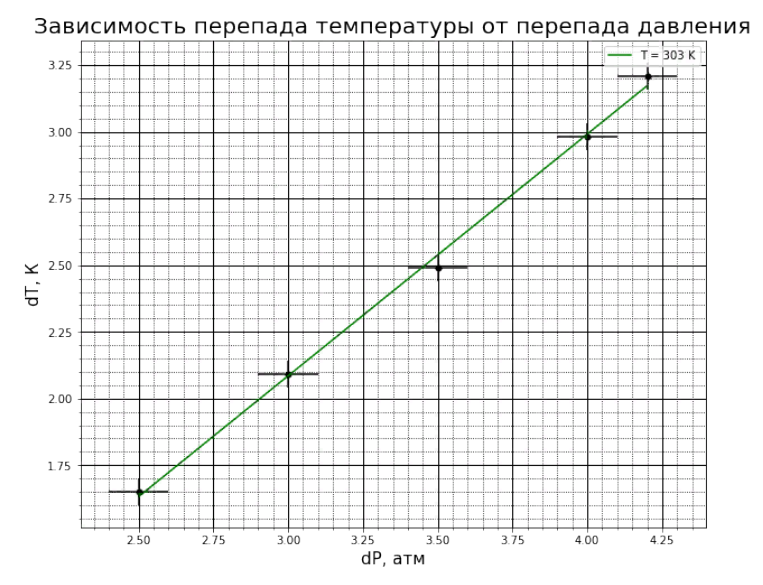
\includegraphics[scale=0.9]{lab216ris3.png}}
\caption{\textit{Зависимость перепада температуры от перепада давления при 303К}}
\end{figure}

\begin{figure}[hbt]
\center{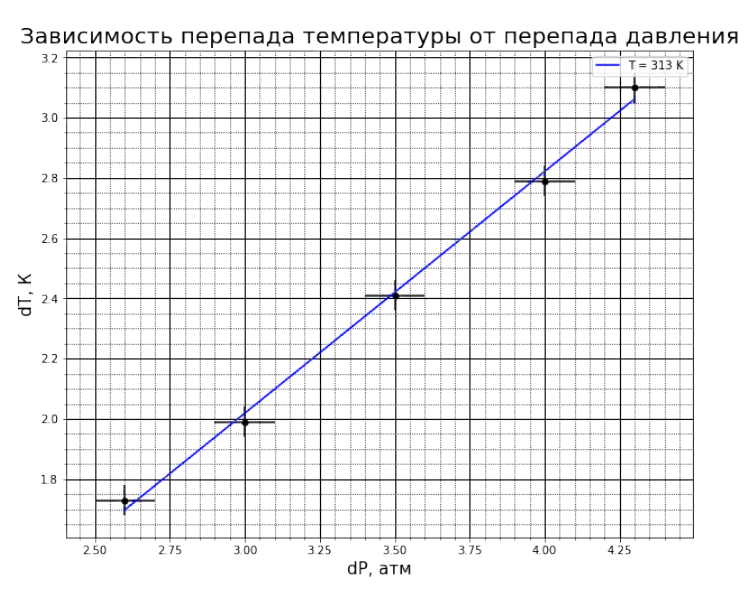
\includegraphics[scale=0.9]{lab216ris4.png}}
\caption{\textit{Зависимость перепада температуры от перепада давления при 313К}}
\end{figure}

\end{document}


